\documentclass[12pt]{extarticle}
\usepackage{fancyhdr}
\usepackage{graphicx}
\usepackage[letterpaper, portrait, margin=1in]{geometry}
\pagestyle{fancy}
\renewcommand{\headrulewidth}{1pt}
\rhead{\textit{Proposal : QoS based Optimal Route Discovery using OpenFlow} \\CSC 573-002}
\usepackage{geometry}

\begin{document}
  \begin{titlepage}
    \vspace*{\fill}
    \begin{center}
{\Huge \textbf{{ QoS based Optimal Route Discovery using OpenFlow }}} \\
      \vspace{20mm}
     \begin{Large}
      Dhaval Sonawane (dsonawa)\\
      Vaibhav Rajadhyaksha (vrajadh)\\
      Elson Serrao (eserrao)\\
      Chethan Nannivala Thipperudrappa (cnanniv)\\
      \vspace{10mm}
      $$9^{th} October, 2015$$
     \end{Large}
    \end{center}
    \vspace*{\fill}
  \end{titlepage}
  
  \newpage
  \vspace{4mm}
\section*{Problem Description}

Routing algorithms traditionally route packets using greedy approach to datagram delivery. Algorithms are broadly classified into Distance Vector and Link State algorithms. The primary metrics used by these algorithms to calculate shortest path is number of hops or the link-cost defined based on the  bandwidth. Essentially when a new shortest path is identified, all the traffic is routed in that direction. Nowhere in this technique do we take the QoS requirements of the traffic into consideration. There may exist cases where a new path is calculated and the traffic is routed to it, even though the old path could still be satisfying the QoS requirements. 

In our project we design a routing scheme based on the QoS requirements of the traffic. We take into consideration link latency, bandwidth and queue/port drops as the QoS metrics to calculate the shortest path based on the service requirement(ToS/DSCP). These metrics are fed to a cost function based on which the shortest path is calculated based on the service requirements.\\


\newpage
\vspace{4mm}
\section*{Components}
{\large \textbf{Platforms for Project}}\\ 
\begin{flushleft}
\textbf{OpenFlow} is a Software Defined Networking (SDN) paradigm that provides centralized control functions by decoupling control and data forwarding layers of routing. \\
\vspace{2mm}
\textbf{GENI} is a national scale sharable network test-bed that allows experimentation with different architectures, fundamentally incompatible. \\
\vspace{2mm}
\textbf{Ubuntu} We will be provisioning Ubuntu machines on GENI to develop/test all our modules.\\
\vspace{2mm}
\textbf{POX} It is an OpenFlow controller which provides APIs in Python. \\

\end{flushleft}
\vspace{4mm}
{\large \textbf{Major components:}}\\
\begin{flushleft}
\textbf{Link Probing Unit : } Link probing unit queries the switch and records the link parameters such as jitter, packet drops in the link state database. This information is further used by “Path Finder” to find the optimal routes. This unit probes the network periodically or upon interrupt by the link or node state change. It periodically collects the link latency information by sending a probe packet to the switch.\\
\vspace{2mm}
\textbf{QoS Index Calculator :} QoS index calculator uses a cost function using the link parameters saved in the LSDB to calculate the QoS index for a particular link. This information is fed to the Path Finder to determine the optimal path.\\
\vspace{2mm}
\textbf{Path Finder :} Path finder is used to calculate the optimal path for each class of traffic based on the input of the QoS Index calculator. Optimal route is calculated periodically/incrementally.\\
\vspace{2mm}
\textbf{Flow Table Modifier :} This uses the entries from the flow database, to update the flow tables in the switches. The updates are non-periodic and are subject to update in entries of the flow database.\\
\vspace{4mm}
Figure (1) and (2) represents the Block Diagram and the Flow Diagram respectively.

\end{flushleft}

\newpage
\begin{center}
\vspace*{\fill}
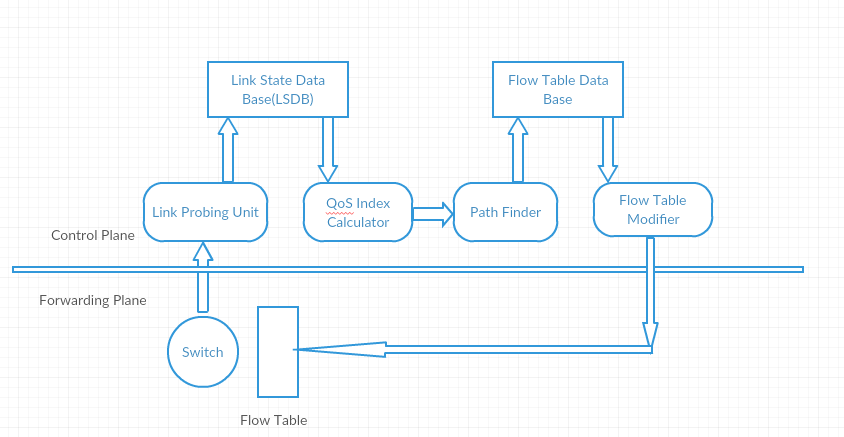
\includegraphics[width=\textwidth]{Block_diagram}
\textit{Figure (1) : Block Diagram}
\end{center}
\vspace*{\fill}

\newpage
\begin{center}
\vspace*{\fill}
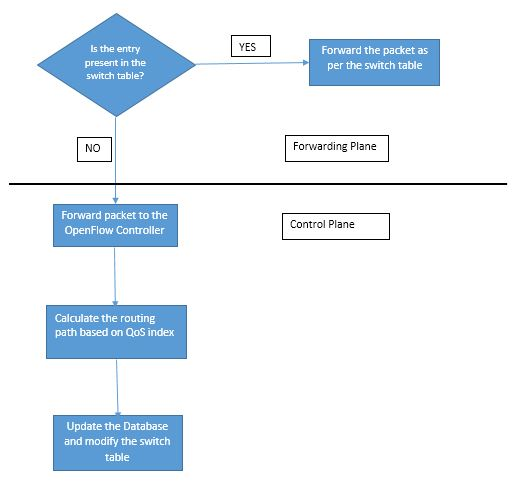
\includegraphics[width=\textwidth]{flow_diagram}
\center \textit{Figure (2) : Flow Diagram}
\vspace*{\fill}
\end{center}

\newpage
\vspace{4mm}
\section*{Demo/Test Plan}
{\large \textbf{Test Environment :} }\\

The test environment consists of:
\begin{itemize}
\item OpenFlow Switches
\item POX based OpenFlow Controller
\item Host nodes to generate traffic using D-ITG (Distributed Internet Traffic Generator) utility.
\end{itemize}

\vspace{3mm}
{\large \textbf{\begin{flushleft}
Testcases:
\end{flushleft}}} 
\vspace{2mm}
Test the adaptive routing/switching functionality by sending the below types of traffic using D-ITG.
\begin{enumerate}
\item Best effort delivery traffic.
\item Single type of Multimedia traffic
\item Multiple type of Multimedia traffic
\item Best effort traffic along with Multimedia traffic.
\end{enumerate}

\end{document}